\documentclass[english,12pt,presentation]{beamer}
\usepackage{graphicx}
\usepackage{beamerthemesplit}
%\setbeameroption{show notes on second screen=right}
\usetheme{EastLansing}
\useinnertheme{circles}
\useoutertheme{infolines}
\usecolortheme{spruce}
\title{Drupal Website Development Using Emacs}
\subtitle{GNU Emacs - Professionals Swiss Army Knife}
\author{Aaron Bello, aaron@hosttor.com, @hosttor}
\date{\today}

\begin{document}
\begin{frame}{Drupal Nights}
\begin{figure}
\centering

\includegraphics[width=80]{images/logo.png}
\end{figure}
\titlepage
\end{frame}

\begin{frame}{What is GNU Emacs?}
\begin{itemize}
\pause \item An integrated enviroment written in Lisp. 
\pause \item Lisp was first developed in the late 50s at MIT for research in artificial intelligence and it is the second-oldest most used programming language toady. 
\pause \item You can do all your work within GNU Emacs including document and file management
\pause \item Supported OS are GNU/Linux, Mac OS X, MS Windows, Solaris
\pause \item Disadvantage of GNU Emacs is high learning curve.
\pause \item Download GNU Emacs at gnu.org/software/emacs
\pause \item Ctrl-h followed by t. For Tutorial
\end{itemize}
\end{frame}

\begin{frame}{Emacs Supported Technologies}
\begin{itemize}
\pause \item HTML, CSS and Javascript
\pause \item Python, Django
\pause \item Java
\pause \item Lisp
\pause \item C or C$++$
\pause \item Arduino
\pause \item Vi/Vim
\pause \item Swift
\pause \item And many more...
\end{itemize}
\end{frame}

\begin{frame}{Thanks to Free Software Foundation}
\begin{figure}
\centering

\includegraphics[width=300]{images/fsf.png}
\end{figure}
\end{frame}

\begin{frame}{Why Emacs For Drupal Development?}
\begin{itemize}
\pause \item Save time and increase productivity
\pause \item The best industry tools for professionals
\pause \item It is Free Software. No licence fees
\pause \item You can modify the source code oppose to what you paid for with limitations.
\pause \item You can share the software among your family, friends and anyone interested in Free Software.
\pause \item Huge community with users worldwide.
\end{itemize}
\end{frame}

\begin{frame}{Powerful Brands Using Drupal}
\begin{figure}
\centering
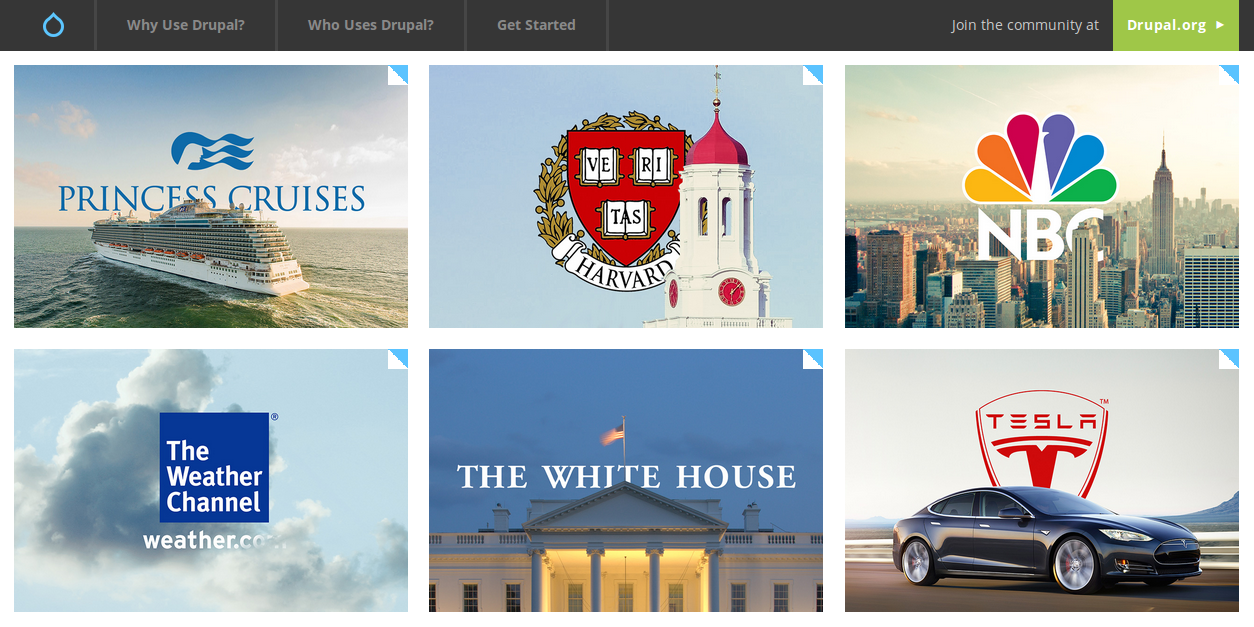
\includegraphics[width=300]{images/drupaluser.png}
\end{figure}
\end{frame}

\begin{frame}{Powerful Brands using Drupal}
\begin{itemize}
\pause \item Stanford Law School
\pause \item Brown University
\pause \item Yale University
\pause \item University of Oxford
\pause \item Bentley University
\pause \item PUMA - PUMA.COM
\pause \item CJ Affliate By Conversant - CJ.COM
\pause \item MassPEP - Massachusetts Pre-Engineering Program
\pause \item The University of Tennessee and other universities
\pause \item Governments, Corporations and Organizations around the world have also adopted Drupal
\end{itemize}
\end{frame}

\begin{frame}{Demostration Time}
\begin{itemize}
\pause \item There are so many packages available to download.
\pause \item Use Alt-x list-packages to see all packages.
\end{itemize}
\begin{figure}
\centering

\includegraphics[width=320]{images/altx.png}
\end{figure}
\end{frame}

\begin{frame}{Demostration Time}
\begin{itemize}
\pause \item org-mode, org-agenda
\pause \item weather, phases-of-moon, dictionary, holiday, chess, doctor, macroc
\pause \item auto-complete, emmet, yasnipet, rainbow, show css
\pause \item weblogger-setup-weblog. Require blogger API. visit abc.com/xmlrpc.php
\pause \item You can create your own package using Emacs Lisp code or GUI.
\end{itemize}
\end{frame}

\begin{frame}{How I Use Emacs}
\begin{itemize}
\pause \item Twitter, IRC, LaTex, secure password, HTML, CSS, PHP, JS
\pause \item SSH, RSYNC, FTP, SCP, etags for Drupal Website
\pause \item Drupal mode is an advanced minor mode for development and management
\pause \item Write code that adheres to drupal coding standards.
\pause \item Search documentation for the symbol at point
\pause \item python, Java, vi/vim, C or C$++$, Lisp, Arduino and many more...
\pause \item Project Showcase: MassPEP Website using Drupal, CiviCRM, Drupal Gap
\end{itemize}
\end{frame}

\begin{frame}{Special Thanks To AGARIC, FSF, BIORAFT, DRUPALNIGHTS, MAYFIRST}
\begin{figure}
\centering

\includegraphics[width=300]{images/specialthanks.png}
\end{figure}
\end{frame}

\begin{frame}{Thank you all for coming}
\item Thank you! Thank you!! Thank you!!!
\end{frame}

\begin{frame}{QUESTIONS?}
\begin{figure}
\centering

\includegraphics[width=300]{images/q.png}
\end{figure}
\end{frame}
\end{document}

